%%%%%%%%%%%%%%%%%%%%%%%%%%%%%%%%%%%
% Basic formatting and settings
%%%%%%%%%%%%%%%%%%%%%%%%%%%%%%%%%%%
\documentclass[12pt,a4paper]{report}
\usepackage[utf8x]{inputenc}
\usepackage[IL2]{fontenc}
\usepackage{a4wide}
\usepackage[left=2cm, right=2cm, top=2.5cm, bottom=2.5cm]{geometry}

%%%%%%%%%%%%%%%%%%%%%%%%%%%%%%%%%%%
% Include required packages
%%%%%%%%%%%%%%%%%%%%%%%%%%%%%%%%%%%
\usepackage{amsmath,amssymb,amsthm}
\usepackage[usenames]{color}
\usepackage{nicefrac}
\usepackage{verbatim}
\usepackage{graphicx}
\usepackage{enumitem}
\usepackage{setspace}
\usepackage{tabularx}
\usepackage{listings}
\usepackage[section]{placeins}

\usepackage[pdftex,bookmarks=true,colorlinks,linkcolor=blue,urlcolor=blue,unicode]{hyperref}
\hypersetup{pdftitle=ODCleanStore}

%%%%%%%%%%%%%%%%%%%%%%%%%%%%%%%%%%%
% Additional formatting settings
%%%%%%%%%%%%%%%%%%%%%%%%%%%%%%%%%%%

%\pagestyle{plain}
\pagestyle{headings}
\linespread{1.1}
\setcounter{secnumdepth}{3}
\setcounter{tocdepth}{2}

%%%%%%%%%%%%%%%%%%%%%%%%%%%%%%%%%%%
% Include macro definitions and package settings
%%%%%%%%%%%%%%%%%%%%%%%%%%%%%%%%%%%

%%%%%%%%%%%%%%%%%%%%%%%%%%%%%%%%%%%
% Indent settings for paragraphs, itemize and enumerate environment
%%%%%%%%%%%%%%%%%%%%%%%%%%%%%%%%%%%
\setitemize{noitemsep,topsep=2pt,leftmargin=30pt}
\setenumerate{noitemsep,topsep=2pt,leftmargin=30pt}
\setdescription{style=sameline}
%\setlength{\parindent}{0pt} % nastavuje odsazení prvniho radku
%\setlength{\parskip}{1.2ex plus 0.5ex minus 0.2ex} % odstup mezi odstavci

\newcommand{\moreindent}{\addtolength{\leftskip}{1.8em}}
\newcommand{\lessindent}{\addtolength{\leftskip}{1.8em}}
\newcommand{\suppressgaps}{\setlength{\parskip}{0pt}}

%%%%%%%%%%%%%%%%%%%%%%%%%%%%%%%%%%%
% Shortcuts for math mode
%%%%%%%%%%%%%%%%%%%%%%%%%%%%%%%%%%%
\newcommand{\coloneqq}{\mathrel{\mathop:}=}
\renewcommand{\O}{{\mathcal{O}}}
\newcommand{\etc}[2]{#1_1,\ldots,#1_#2}
\def\<#1>{\leavevmode\hbox{\it #1\/}} % usage: \<variable>

%%%%%%%%%%%%%%%%%%%%%%%%%%%%%%%%%%%
% Other shortcuts and style commands
%%%%%%%%%%%%%%%%%%%%%%%%%%%%%%%%%%%
\newcommand{\quot}[1]{``#1''}
\newcommand{\code}[1]{\texttt{#1}}
\newcommand{\varcode}[1]{\textit{\textless #1\textgreater}}
\newcommand{\vartext}[1]{\textit{#1}}
\newcommand{\tab}{\rule{30pt}{0pt}}
\newcommand{\term}[1]{\textit{#1}}
\newcommand{\todo}[1]{}
\newcommand{\importantterm}[1]{\textbf{#1}}

% These macros use a dirty trick to persuade LaTeX to typeset chapter headers
% more readably and not to leave plenty of space above them.
\makeatletter
\def\@makechapterhead#1{
  {\parindent \z@ \raggedright \normalfont
   \Huge\bfseries \thechapter. #1
   \par\nobreak
   \vskip 20\p@
}}
\def\@makeschapterhead#1{
  {\parindent \z@ \raggedright \normalfont
   \Huge\bfseries #1
   \par\nobreak
   \vskip 20\p@
}}
\makeatother

% Chapter that is not numbered but included in the contents
\def\chapwithtoc#1{
\chapter*{#1}
\addcontentsline{toc}{chapter}{#1}
} 

\newenvironment{enumeratei}
	{
		\begin{enumerate}
		\renewcommand{\labelenumi}{(\textit{\roman{enumi}})}
	}
	{
		\end{enumerate}
	}

\newenvironment{glossarylist}
	{\begin{description}[style=nextline,itemsep=8pt]}
	{\end{description}}

\newenvironment{configlist}
	{\begin{description}[style=nextline,font=\ttfamily]}
	{\end{description}}

\newenvironment{dirlist}
	{\begin{description}[style=sameline,font=\ttfamily]}
	{\end{description}}
	
%%%%%%%%%%%%%%%%%%%%%%%%%%%%%%%%%%%
% Package settings
%%%%%%%%%%%%%%%%%%%%%%%%%%%%%%%%%%%%

% lstlistings environment
% Defines a custom trivlisting environment
\lstset{basicstyle=\ttfamily\footnotesize,columns=flexible,
  frame=lines,float=ht,captionpos=b,aboveskip=1.5\bigskipamount}
\lstnewenvironment{trivlisting}
  {\lstset{basicstyle=\ttfamily,aboveskip=\medskipamount,frame=none}}
  {}

%%%%%%%%%%%%%%%%%%%%%%%%%%%%%%%%%%%
% Document-specific commands
%%%%%%%%%%%%%%%%%%%%%%%%%%%%%%%%%%%
\newcommand{\refusermanual}{User Manual\xspace}
\newcommand{\refadminmanual}{Administrator's \& Installation Manual\xspace}
\newcommand{\refprogrammersguide}{Programmer's Guide\xspace}
\newcommand{\configdefault}[1]{\newline\textit{Default value:}~\code{#1}}
\newcommand{\odcs}{ODCleanStore\xspace}
\newcommand{\reqparagraph}[1]{\paragraph{\textnormal{\textit{#1}}}}

%%%%%%%%%%%%%%%%%%%%%%%%%%%%%%%%%%%
% Aligned enumeration tables
%%%%%%%%%%%%%%%%%%%%%%%%%%%%%%%%%%%
\newcommand{\enumtable}[1]
{
	\begin{table}[!ht]
		\begin{tabularx}{\linewidth}{>{\textbf\bgroup}l<{\egroup}X}
			#1
		\end{tabularx}
	\end{table}
}

%%%%%%%%%%%%%%%%%%%%%%%%%%%%%%%%%%%
% Aligned field description tables
%%%%%%%%%%%%%%%%%%%%%%%%%%%%%%%%%%%
\newcommand{\fieldtable}[1]
{
	\begin{table}[!ht]
		\begin{tabularx}{\linewidth}{|>{\textbf\bgroup}l<{\egroup}|p{3cm}|X|}
			\hline
			\textnormal{Required} & Field & Description \\
			\hline \hline
			#1 \\
			\hline
		\end{tabularx}
	\end{table}
}


%%%%%%%%%%%%%%%%%%%%%%%%%%%%%%%%%%%
% Optionally disable use of images.
% Convenient for export to .dvi when the documents contain images not supported in plain latex
% Uncomment to disable images.
%%%%%%%%%%%%%%%%%%%%%%%%%%%%%%%%%%%
%\renewcommand{\includegraphics}[2][1]{}

\newcommand{\version}{0.3.6}
\newcommand{\documentname}{\refprogrammersguide}


\begin{document}

\title{ODCleanStore -- \documentname}

\begin{titlepage}
\begin{center}

\large
Charles University in Prague

\smallskip

Faculty of Mathematics and Physics

%\vspace{\stretch{1}}
%{\bf\Large SOFTWARE PROJECT}

\vspace{\stretch{3}}

\resizebox{0.5\linewidth}{!}{\bf\Huge ODCleanStore}

%\bigskip
%\resizebox{0.3\linewidth}{!}{Open Data store}

\vspace{\stretch{3}}
\begin{spacing}{1.5} 
{\bf\Huge \documentname}
\end{spacing}

\vspace{\stretch{1}}
Release \version\\
\today

\vspace{\stretch{15}}

\begin{tabular}{rl}

\textbf{Authors:} & Jan Michelfeit \\
& Du\v san Rychnovsk\'y\\
& Jakub Daniel\\
& Petr Jerman\\
& Tom\' a\v s Soukup\\
\noalign{\vspace{3mm}}
\textbf{Supervisor:} & RNDr. Tom\' a\v s Knap
\end{tabular}

\end{center}
\end{titlepage}

\newpage

\renewcommand{\contentsname}{Contents}
\tableofcontents
\bigskip

\newpage

%%%%%%%%%%%%%%%%%%%%%%%%%%%%%%%%%%%%%%%%%%%%%%%%%%%%%%%%%%%%%%%%%%%%%%%%%%%%%%

% !List of features and intended use-cases (zduvodneni featur FE)
	% rrequirements - functional, intraface, non-functional?


% release proces
% issues redmine - debugging & spol
% used technologies
% FE
	% zdokumentovat, co je potřeba pro přidání DN template apod.
  % FE - popsat, že to je webová aplikace, dá se spouštět pod tomcatem, odkaz na install manual
  % význam abstraktních Dao
  % uncommitted tabulky
  % jak přidat novou stránku


	% třídy
		% webfrontend.behavior - Wicket Behavior implementations
		% webfrontend.bo
		% webfrontend.configuration
		% webfrontend.core
			% DaoLookupFactory, ODCSWebFrontendApplicatoin .java/properties, ODCSWebFrontendSession, URLRouter
		% webfrontend.core.components - custom Wicket components (buttons, labels, form components etc.)
		% webfrontend.core.model - Wicket models and data providers
		% webfrotend.dao
		% webfrontend.pages - pages, panels, ...
		% webfrontend.util
		% webfrontend.validators

	% naming conventions

%%%%%%%%%%%%%%%%%%%%%%%%%%%%%%%%%%%%%%%%%%%%%%%%%%%%%%%%%%%%%%%%%%%%%%%%%%%%%%

\chapter{Introduction}
\odcs is a~server application for management of Linked Data written in Java. It stores data in RDF, processes them and provides integrated views on the data.

This document serves as the main documentation for developers. It describes basic architecture, implementation, development process, used technologies and other important information relevant for people who want to participate in the development of \odcs.

\section{What is ODCleanStore}
\odcs accepts arbitrary RDF data and metadata through a SOAP webservice (\term{Input Webservice}). The data is processed by \term{transformers} in one of a~set of customizable \term{pipelines} and stored to a~persistent store (OpenLink Virtuoso database instance). The stored data can be accessed again either  directly through a SPARQL endpoint or through \term{Output Webservice}. Linked Data consumers can send queries and custom query policies to Output Webservice and receive (aggregated/integrated) RDF data relevant for their query, together with information about provenance and data quality. 

\section{Related documents}
More detailed information about \odcs from the perspective of a user or an administrator can be found in related documents \quot{\refusermanual} and \quot{\refadminmanual}. \refusermanual also contains definition of user roles, glossary of terms etc.

Other working documents related to development are located at the project's page at SourceForge\footnote{\url{https://sourceforge.net/p/odcleanstore/wiki/For\%20developers/}}. The Wiki tool at SourceForge is used for working documents, discussion of new features, description of testing scenarios etc. Not all pages are up-to-date, however, and this document is authoritative in case of conflicts.

%%%%%%%%%%%%%%%%%%%%%%%%%%%%%%%%%%%%%%%%%%%%%%%%%%%%%%%%%%%%%%%%%%%%%%%%%%%%%%
%\chapter{Requirements}
% todo
% features, interfaces, administration, future use
% motivace, ostatní existující řešení, v čem je to nové


%%%%%%%%%%%%%%%%%%%%%%%%%%%%%%%%%%%%%%%%%%%%%%%%%%%%%%%%%%%%%%%%%%%%%%%%%%%%%%
\chapter{ODCleanStore overview} 
An overview of how \odcs works is depicted on \figurename~\ref{fig:odcsInternal}.

\begin{figure}[htb]
    \centering
    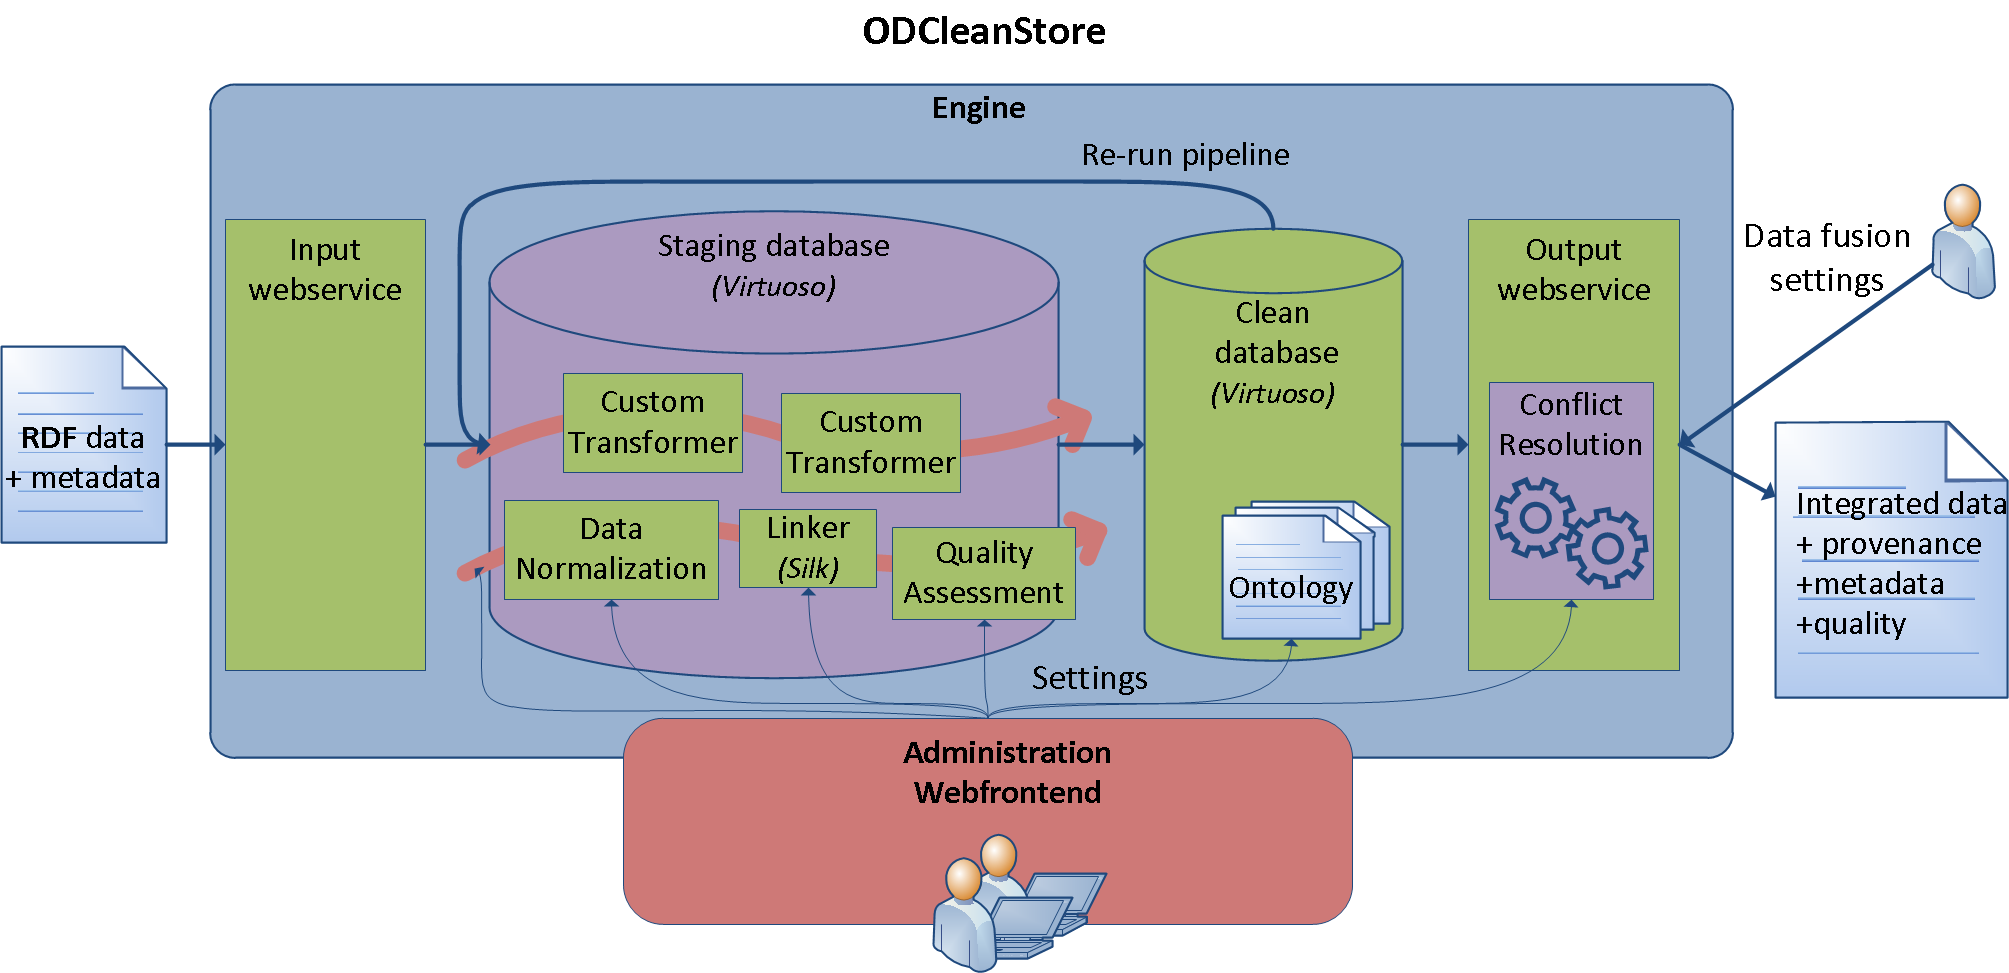
\includegraphics[width=\textwidth]{images/odcs-internal.png}
    \caption{Overview of ODCleanStore architecture}
	\label{fig:odcsInternal}
\end{figure}

The diagram lists all main functional units in \odcs:

\begin{itemize}
	\item \importantterm{Engine.}
		Engine runs the whole server part. It realizes all data processing and starts Input and Output Webservices.

		\begin{itemize}
			\item \importantterm{Input Webservice}. SOAP webservice that accepts new data and queues them for processing in the dirty database.
			\item Pipeline processing. Processes queued data by running a series of transformers in a pipeline on it and moves the dat to the clean database.
			\item \importantterm{Ouptut Webservice}. REST webservice for querying over data in the clean database.
		\end{itemize}
	\item \importantterm{Query Execution \& Conflict Resolution.}
		\QE retrieves all data and metadata relevant for a query asked via Output Webservice. Conflict Resolution then resolves conflicts in the retrieved data, including resolution of \code{owl:sameAs} links.
	\item Predefined transformers.
		Transformers used for data processing that are included by default in \odcs.
		\begin{itemize}
			\item \importantterm{Quality Assessment}. Estimates quality of data based on user-defined or generated rules.
			\item \importantterm{Data Normalization}. Transformations of data based on user-defined or generated rules.
			\item \importantterm{Linker}. Generates links (e.g. \code{owl:sameAs}) between resources in the processed data and contents of the clean database.
			\item Other transformers -- Other transformers such as Quality Aggregator, Blank Node Remover etc.
		\end{itemize}
	\item \importantterm{Administration Frontend.}
		Web application written in Java from which \odcs can be managed. In Administration Frontend, the user can define pipelines for data processing, rules for transformers, manage ontologies, Output Webservice settings etc.
\end{itemize}

Each of these parts will be described later in this document. In the source code, the components are divided into several maven projects described in Section \ref{sec:mavenBuild}.

\section{Important concepts}
\odcs is about data. More specifically, it works with data represented in RDF\footnote{\url{http://www.w3.org/TR/2004/REC-rdf-primer-20040210/}}. \odcs implements three tasks regarding data:

\begin{enumerate}
	\item Data processing
	\item Storing data
	\item Querying over stored data
\end{enumerate}

\subsection{Data Processing}
Data processing is realized by \term{transformers} that are applied to data being processed by Engine in a \term{pipeline}. A transformer can be any class implementing the \code{Transformer} interface but typically it only manipulates (change, add, delete) processed data in database. Several transformers ship with \odcs, such as Quality Assessment, Linker or Data Normalization.

It is important to distinct between a \term{transformer} and \term{transformer instance}. By \term{transformer}, we mean the Java class which implements the \code{Transformer} interface and is registered in ODCleanStore administration (managed by users in role Administrator). \term{Transformer instance} is assignment of such transformer to a pipeline. For example, the Quality Assessment transformer is registered in ODCleanStore by default. The user can create two pipelines and assign the Quality Assessment transformer to each of them, thus creating two transformer instances.

Some transformers can be configured in Administration Frontend by \term{rules}. In general, these rules are grouped to \term{rule groups}. Rule groups can be then assigned to transformer instances.

See also Section \ref{sec:dataLifecycle} \nameref{sec:dataLifecycle}.

\subsection{Storing Data}
Data are stored using Open Link Virtuoso RDF database. Two instances of this database are used for every deployment of \odcs:

\begin{itemize}
	\item \term{Dirty (staging) database} -- contains data that are currently being processed. Contents of this instance is not directly visible for data consumers (users in role USR).
	\item \term{Clean database} -- contains already processed data that are accessible through the Output Webservice to data consumers (users in role USR).
\end{itemize}

\subsection{Querying over Stored Data}
Querying over stored data is realized by Output Webservice which supports several types of queries (see \refusermanual). For retrieval of results and resolving conflicts, Output Webservice uses components \QE (Section \ref{sec:QE}) and Conflict Resolution (Section \ref{sec:CR}).

\subsection*{}

See also Glossary in Appendix \ref{chap:glossary} for explanation of important concepts.

\section{Data Lifecycle}
\label{sec:dataLifecycle}

The lifecycle of data inside \odcs is as follows:

\begin{enumerate}
  \item RDF data (and additional metadata) are accepted by Input Webservice and stored as a~named graph to the {dirty database}. Data can be uploaded by any third-party application registered in \odcs.
  \item Engine successively processes named graphs in the dirty database by applying a~pipeline of transformers to it; the applied pipeline is selected according to the input metadata.
  \item Each transformer in the pipeline may modify the named graph or attach new related named graphs (such as a named graph with mappings to other resources or results of quality assessment).
  \item When the pipeline finishes, the augmented RDF data are populated to the {clean database} together with any auxiliary data and metadata created during the pipeline execution.
  \item Data consumers can use Output Webservice to query data in the clean database. Output Webservice provides several basic types of queries -- URI query, keyword and named graph query; in addition, metadata about a~given named graph can be requested. The response to a~query consists of relevant RDF triples together with their provenance information and quality estimate. The query can be further customized by user-defined conflict resolution policies.\\
	Data in the clean database can be also queried using the SPARQL query language. While SPARQL queries are more expressive, there is no direct support for provenance tracking and quality estimation. 
  \item When transformer rules change, the administrator may choose to re-run a~pipeline on data already stored in the clean database. Copy of this data is created in the dirty database where it is processed by the pipeline. After that, the processed version of data replaces the original in the clean database.
\end{enumerate}

%%%%%%%%%%%%%%%%%%%%%%%%%%%%%%%%%%%%%%%%%%%%%%%%%%%%%%%%%%%%%%%%%%%%%%%%%%%%%%
\chapter{Implementation}
\section{Architecture}

\subsection{Architecture Evolution}
The architecture that is depicted on \figurename~\ref{fig:odcsInternal} was chosen for several reasons.

First, the division into components is natural with regard to the original specification of the software project. All important components are included and we have also kept other concepts, such as two dataspaces for clean and dirty data, or the flexibility of data-processing pipeline.

Second, the selected architecture allowed a clear division of work and enabled a relative independence of each component.

Third, it is a result of a long process of analysis. From the initial vision and  requirements specification, which suggested an abstract concept of tranformers run in arbitrary order on data, we extracted several most important cases of transformers that were tightly bound to the system and could run only in a fixed order, only to generalize them back to transformers with a~very simple interface and flexible pipelines.


\subsection{Architectural Features}

\subsubsection{Components}
\odcs consists of several components that are (mostly) loosely-coupled only through a simple interface specified in advance. This made it easy divide tasks among developers and enabled them to work independently.

\subsubsection{Internal Interfaces}
In order to minimize interfaces between parts of \odcs, to minimize system requirements and to make the system more robust, we decided to prefer communication through data shared in database.

There is no direct interface between Engine and Administration Frontend, but the Administration Frontend saves all configuration to a relational database from which the Engine can retrieve it. This enbles updates of settings in transactions, prevents synchronization issues and enables the two parts to run completely independendently (even on separate machines).

Transformers run in a pipeline are isolated and don't know about each other. Instead of passing data to be transformed through an interface in memory, only the names of named graphs where data are stored are passed to each transformer. This enables to write transformers that are oblivious to \odcs as much as possible and only need to work with data by manipulating the database. Also, it gives transformers the full power of the SPARQL/SPARUL language. Although we should note that in practice, the transformer implementation may be tied with the use of Virtuoso as the underlying database, this is not such a downside because Virtuoso is one of the most popular RDF databases.

\subsubsection{Interoperability}
The external interfaces are implemented using standard technologies (SOAP for Input Webservice, REST for Output Webservice) and standard formats (RDF/XML, Turtle/Notation3). This should minimize the effort for integration with third-party applications communicating with \odcs. We also provide a Java library for accessing the Input Webservice to futher minimize the effort.

\subsubsection{Used Technologies}
The choice of Java for implementation and Virtuoso as the underlying database ensure platform independence.

Since Java is a very wide-spread language, \odcs can be extended with minimum effort for learning new technologies (e.g. when adding new transformers).

\subsubsection{Scalability}
 Although currently the Engine is processing data sequentially, it is designed for parallel processing in the future. It could even be extended to work in a distributed manner on several machines.

 Most of the work the Input Webservice has is with data processing in pipelines. Since pipelines can run independently, each Engine instance could even use a dedicated database instance for dirty data.

 On the other hand, the Output Webservices uses the clean database in a read-only manner and thus could be also deployed on several database instances if database replication is put in place.

\section{Other requirements}
The assignment of the project impose several additional requirements. This section lists how they were satisfied.

\reqparagraph{It should be easy to incorporate other components, such as a component computing popularity of the data sources.} This requirement is satisfied with the introduction of custom transformers.

\reqparagraph{The application will involve graphical user interface enabling management of all kinds of policies etc.} Administration Frontend enables management of all relevant settings. In addition, several user roles are supported and user accounts can be managed from Administration Frontend.

\reqparagraph{The application will run at least on Windows 7, Windows Server 2008, Linux.} \odcs requires Java Runtime Environment and Virtuoso installation, both supported on all of the listed platforms. \odcs has been tested on Windows 7, Windows Server 2008 and Debian distribution of Linux.

\reqparagraph{Application will be freely available under Apache Software License.} \odcs is published under the required license (see \refadminmanual) and source codes available at a public repository at SourceForge.net

\section{Used technologies}
The chosen language for implementation is Java. The reason is that there are many libraries and tools required for implemenation accessible in Java, it enables platform independence (one of the requirements on \odcs) and also it is very wide-spread so that developers don't need to learn a new syntax.

\subsection{Database}
Openlink Virtuoso\footnote{\url{http://virtuoso.openlinksw.com/}} is used as the underlying data store. It is the most popular RDF storage with a solid support. Both a commercial version and Open Source edition\footnote{\url{http://virtuoso.openlinksw.com/dataspace/dav/wiki/Main/}} exists.

RDF data store provided by Virtuoso supports reasoning, most notably \code{owl:sameAs} link resolution, which proved essential for Query Execution/Conflict Resolution components. Virtuoso also provides a relational database which relieves us from the need of another database for that purpose.

The downside is somewhat buggy behavior (especially SPARQL query parsing) and lack of working support for transactions with RDF data.

\subsection{Administration Frontend}
Apache Wicket\footnote{\url{http://wicket.apache.org/}} is used for implemenation of the Administration Frontend. It is a component system for writing web applications in Java. Advantages are proper mark-up and logic separation, POJO data model and rapid development of this particular type of web application. Wicket was also chosen by our sister project Strigil\footnote{\url{http://strigil.sourceforge.net/}} so a more tight integration of the two tools may be possible in the future.

Spring\footnote{\url{http://www.springsource.org/}} is used for simplified access to the relational database and transaction management. Use of Hibernate\footnote{\url{http://www.hibernate.org/}} for the DAO layer was rejected because of problems with integration with Wicket.

\subsection{Libraries}
\subsubsection*{Jena}
Apache Jena\footnote{\url{http://jena.sourceforge.net/}} is a library for manipulation with RDF data. It supports represenation of RDF data in memory, parsing, loading and updating of RDF models. In \odcs, it is used mainly for representation of RDF triples (quads) and serialization of RDF, because other features proved problematic when used with large data.

We chose Jena over its alternative Sesame\footnote{\url{http://www.openrdf.org/}} because it supports working with named graphs through NG4J and we had previous experience with it.

\subsubsection*{NG4J}
NG4J\footnote{\url{http://wifo5-03.informatik.uni-mannheim.de/bizer/ng4j/}} extends Jena with named graphs API.

\subsubsection*{SLF4J}
SLF4J\footnote{\url{http://www.slf4j.org/}} is a flexible and efficient library used for logging. 

\subsection{Development tools}
\subsubsection*{Maven}
Apache Maven\footnote{\url{http://maven.apache.org/}} is used as the build tool. It was chosen over Apache Ant because Maven saves work with its many available plugins (such as Maven Jetty Plugin) and offers simple management of dependencies.

\subsubsection*{Git}
Git is used as the version control system. We used it because it enables simple manipulation with branches and merging but most importantly it is less dependent on a central server whose potential unavailability was identified as a potential risk.



%%%%%%%%%%%%%%%%%%%%%%%%%%%%%%%%%%%%%%%%%%%%%%%%%%%%%%%%%%%%%%%%%%%%%%%%%%%%%%
\chapter{Setting up Development Environment}

\section{Quick Start}
\subsection{Tools}
	In order to to prepare environment for building \odcs, first make sure to have installed all necessary tools:

\begin{itemize}
	\item Java Development Kit\footnote{\url{www.oracle.com/technetwork/java/javase/downloads/}} version 6 or newer
	\item Git version control system\footnote{\url{http://git-scm.com/}}
	\item Apache Maven\footnote{\url{http://maven.apache.org/}}
\end{itemize}

Also, make sure you have all the binaries used in the following steps on your classpath. 

\subsection{Obtaining sources} 
\odcs sources are hosted at SourceForge.\footnote{\url{http://sourceforge.net/p/odcleanstore/code/}} Use git to check out the sources:

\begin{verbatim}
      git clone git://git.code.sf.net/p/odcleanstore/code odcleanstore-code
\end{verbatim}

The above command will create a local clone of the repository in \code{odcleanstore-code} directory.

\subsection{Building binaries}
Move to directory \code{odcleanstore} within your local clone of the repository which contains the root maven project (\code{pom.xml}). Then build the project using maven:

\begin{verbatim}
      cd odcleanstore-code/odcleanstore
      mvn clean package install
\end{verbatim}

After that, Engine binaries can be found in directory \code{odcleanstore/engine/target} and the WAR file of Administration Frontend at \code{odcleanstore/webfrontend/target}. Now you can deploy the application as described in \refadminmanual. \todo{jestli tam bude jenom popis instalatoru, mel by se rucni deploy popsat tady a pridat referenci na instalaci Virtuosa}

\section{Repository structure}
\subsection{Branches}
There are several branches in the git repository. The latest development version of is on branch \code{master}. Then there are release branches for each release named \code{release-0.1.x}, \code{release-0.2.x} etc. which contain stable versions for  releases  packages. Each commit that where used to prepeare a release package is labeled with a tag \code{release}-\varcode{version}. Finally, there are feature branches prefixed with \code{feature-}.

Common development takes place on branch \code{master}. New feature branches are created for features that may or may not be accepted or that need time to be finished before they are applied to \code{master}. When whey are finished, they are merged to \code{master} and the branch may be removed in time. Release branches stem from \code{master} for every new major release. Fixes and modifications for minor releases take place on release branches and may be merged from/to \code{master}.

\subsection{Directory structure}
This is an outline of directory structure in the git repository:

\begin{dirlist}
	\item[data/] \mbox{}
		\begin{dirlist}
			\item[initial\_db\_import/] -- database import files
				\begin{dirlist}
					\item[clean\_db/] -- SQL files to be imported to the clean database
					\item[dirty\_db/] -- SQL files to be imported to the dirty database
				\end{dirlist}
			\item[odcs\_configuration/] -- the default \odcs configuration file
			\item[virtuoso\_configuration/] -- configuration files for Virtuoso database instances
		\end{dirlist}
	\item[doc/] -- documentation sources (in \LaTeX)
	\item[odcleanstore/] -- Java sources
		\begin{dirlist}
			\item[backend/] -- sources of \code{odcs-backend} artifact (transformers, Query Execution, Conflict Resolution)
			\item[comlib/] -- sources of \code{odcs-comlib} artifact (code related to sending data to Input Webservice)
			\item[conf/] -- configuration files for development in Eclipse
			\item[core/] -- sources of \code{odcs-core} artifact (common code shared by other artifacts)
			\item[engine/]  -- sources of \code{odcs-engine} artifact (Engine component)
			\item[inputclient/]  -- sources of \code{odcs-imputclient} artifact (Java client for Input Webservice)
			\item[simplescraper/]  -- simple Input Webservice import tool
			\item[simpletransformer/]  -- example of a custom transformer
			\item[webfrontend/]  -- sources of Administration Frontend
			\item[pom.xml] -- the root maven POM file
		\end{dirlist}
\end{dirlist}


\section{Maven build}
\label{sec:mavenBuild}
The project is divided into several artifacts. The root POM (\code{pom.xml}) in \code{odcleanstore} directory defines the parent project while each component of \odcs is in a separate artifact in subdirectories of \code{odcleanstore}. These artifacts are:

\begin{itemize}
	\item \code{odcs-core} -- common code shared by other artifacts; also defines interfaces for custom transformers
	\item \code{odcs-backend} -- predefined transformers, Query Execution and Conflict Resolution
	\item \code{odcs-engine} -- Engine component (running Input and Output Webservice and the data processing queue)
	\item \code{odcs-comlib} -- components shared by \code{odcs-inputclient} and Input Webservice
	\item \code{odcs-webfrontend} -- Administration Frontend web application
	\item \code{odcs-inputclient} -- client library for Input Webservice (provides a Java API for accessing the webservice)
	\item \code{odcs-simplescraper} -- a simple command-line tool for importing data through Input Webservices
	\item \code{odcs-simpletransformer} -- example of a custom transformer
\end{itemize}


It is recommended to always build using the root POM. Building from subprojects may require issuing \code{mvn install} on the root POM first. The entire project can be build with the following command:

\begin{verbatim}
      cd odcleanstore-code/odcleanstore
      mvn clean package
\end{verbatim}

There are two profiles in addition to the default one in the root POM.

\begin{itemize}
	\item \code{javadoc} profile -- enables generation of javadoc (which is disabled in the default profile). 
	\item \code{systest} profile -- enables unit tests in \code{systest/} subdirectories, which test functionality related to the database. In order to run these tests, a new Virtuoso instance with settings as in \code{/data/virtuoso\_configuration/virtuoso.ini-test} must be set up first. \todo{ref to Virtuoso installation guide}
\end{itemize}

Maven build for the selected profile can be executed with command line option \code{-P}:

\begin{verbatim}
      mvn clean package -P javadoc
      mvn clean package -P systest	
\end{verbatim}

%%%%%%%%%%%%%%%%%%%%%%%%%%%%%%%%%%%%%%%%%%%%%%%%%%%%%%%%%%%%%%%%%%%%%%%%%%%%%%
\chapter{Common code}

%%%%%%%%%%%%%%%%%%%%%%%%%%%%%%%%%%%%%%%%%%%%%%%%%%%%%%%%%%%%%%%%%%%%%%%%%%%%%%
\chapter{Engine}

\todo{jak se to spousti, vypina, celkova architektura}

\section{Pipeline Processing}

\section{Input Webservice}

\section{Output Webservice}

\subsection{Output Formatters}

%%%%%%%%%%%%%%%%%%%%%%%%%%%%%%%%%%%%%%%%%%%%%%%%%%%%%%%%%%%%%%%%%%%%%%%%%%%%%%
\chapter{Query Execution}
\label{sec:QE}

\section{Purpose}
The purpose of \QE is to retrieve result for a query (asked through Input Webservice), resolve conflicts using the Conflict Resolution component and return result.

Triples that \QE retrieves are:
\begin{enumerate}
	\item \label{item:queryTriples} Triples relevant for the query (e.g. containing the given URI).
	\item Triples with metadata about named graphs containing triples from (\ref{item:queryTriples}).
	\item Triples containing human-readable labels for URI resources occuring in triples from (\ref{item:queryTriples}).
\end{enumerate}
A special case is the metadata query which retrieves only named graph metadata.

Because the result of conflict resolution depends on the data it is given, \QE and \CR are not independent but rather \QE extracts exactly the data that \CR needs and calls it directly.

\section{Interface}
The public interface of the \QE component is represented by class \code{QueryExecution}.

 This class exposes methods for executing all kinds of supported queries and returns result as an instance of \code{MetadataQueryResult} (wraps collection of provenance metadata triples and other metadata) or \code{BasicQueryResult} (wraps collection of \code{CRQuad}s returned from \CR plus metadata). The query can be further parametrized by passing \code{QueryConstraintSpec} and \code{AggregationSpec} affecting the retrieved data and the conflict resolution process, respectively.

\section{Implementation}
The actual implementation is in classes inheriting from \code{QueryExecutorBase}, each implementing one type of query: \code{URIQueryExecutor}, \code{KeywordQueryExecutor}, \code{NamedGraphQueryExecutor} and \code{MetadataQueryExecutor}. These classes are called internally from the \code{QueryExecution} class.

For each query, the following steps are executed: input is validated, result quads retrieved from the database, metadata and labels are retrieved from the database and conflict resolution is applied to the result.

To improve performance, values that are used for each query but rarely changed are cached. Cached values are: default aggregation settings, prefix mappings and label properties.

\section{Extending}
In order to implement a new type of query, the following steps should be taken:

\begin{enumerate}
	\item Create a class implementating the new query, preferably inheriting from \code{QueryExecutorBase}.
	\item Extend \code{QueryExecution} class with method for executing the query.
	\item Extend Input Webservice to provide access to the new query for users.
\end{enumerate}

\section{Database}
\QE retrieves RDF data from the clean database instance. Because Virtuoso doesn't fully support transactions with RDF data, the clean database may contain incomplete data partially inserted by Engine. In order to filter such data from the result, \QE ignores all named graphs whose URI starts with an agreed prefix\footnote{\code{http://opendata.cz/infrastructure/odcleanstore/internal/hiddenGraph/}} given by Engine to such named graphs.

In addition, \QE loads settings from the following tables in relational database (see Appendix \ref{chap:reldb}):

\begin{itemize}
	\item \dbodcs{qe\_label\_properties}
	\item \dbodcs{cr\_properties} 
	\item \dbodcs{cr\_settings} 
	\item and tables referenced from tables above
\end{itemize}

\todo{zmínka o engine prefixu}

%%%%%%%%%%%%%%%%%%%%%%%%%%%%%%%%%%%%%%%%%%%%%%%%%%%%%%%%%%%%%%%%%%%%%%%%%%%%%%
\chapter{Conflict Resolution}
\label{sec:CR}

%%%%%%%%%%%%%%%%%%%%%%%%%%%%%%%%%%%%%%%%%%%%%%%%%%%%%%%%%%%%%%%%%%%%%%%%%%%%%%
\chapter{Transformers}

\section{Custom Transformers}
\todo{co by měly dodržovat - nešahat do čisté db, transakce, registrovat grafy, nesahat jinam do špinavé db atd.}
\section{Quality Assessment \& Quality Aggregator}
\section{Data Normalization}
\section{Linker}
\section{Other Transformers}
\subsection{Blank Node Remover}
\subsection{Last Update Marker}
\subsection{Property Filter}

%%%%%%%%%%%%%%%%%%%%%%%%%%%%%%%%%%%%%%%%%%%%%%%%%%%%%%%%%%%%%%%%%%%%%%%%%%%%%%
\chapter{Administration Frontend}

\todo{authorization system}

%%%%%%%%%%%%%%%%%%%%%%%%%%%%%%%%%%%%%%%%%%%%%%%%%%%%%%%%%%%%%%%%%%%%%%%%%%%%%%
\chapter{(Conclusion, evaluation)}

%%%%%%%%%%%%%%%%%%%%%%%%%%%%%%%%%%%%%%%%%%%%%%%%%%%%%%%%%%%%%%%%%%%%%%%%%%%%%%
\chapter{(Testing scenario)}
\todo{Do uzivatelskeho manualu?}

%%%%%%%%%%%%%%%%%%%%%%%%%%%%%%%%%%%%%%%%%%%%%%%%%%%%%%%%%%%%%%%%%%%%%%%%%%%%%%
\chapter{(Related Work)}

%%%%%%%%%%%%%%%%%%%%%%%%%%%%%%%%%%%%%%%%%%%%%%%%%%%%%%%%%%%%%%%%%%%%%%%%%%%%%%
\chapter{Future Work}
\todo{plus known bugs?}

%%%%%%%%%%%%%%%%%%%%%%%%%%%%%%%%%%%%%%%%%%%%%%%%%%%%%%%%%%%%%%%%%%%%%%%%%%%%%%
\chapwithtoc{References}


%%%%%%%%%%%%%%%%%%%%%%%%%%%%%%%%%%%%%%%%%%%%%%%%%%%%%%%%%%%%%%%%%%%%%%%%%%%%%%

\appendix

\chapter{Glossary}
\label{chap:glossary}
\section*{RDF-related}
\begin{glossarylist}
	\item[RDF] Resource Description Framework, a~language for representing information about resources in the World Wide Web\footnote{\url{http://www.w3.org/RDF/}}
	\item[RDF triple] Statement about a~resource expressed in the form of subject-predicate-object expression
	\item[URI] Uniform Resource Identifier, identifies RDF resources
	\item[Named graph] A~set of related RDF triples (RDF graph) named with a~URI\footnote{\url{http://www.w3.org/2004/03/trix/}}
	\item[RDF quad] An RDF triple plus named graph URI (subject, predicate, object, named graph)
	\item[Ontology] Representation of the meaning of terms in a~vocabulary and of their interrelationships
	\item[OWL] The Web Ontology Language\footnote{\url{http://www.w3.org/TR/owl-features/}}
	\item[SPARQL] RDF query language\footnote{\url{http://www.w3.org/TR/rdf-sparql-query/}}
	\item[RDF/XML] An XML-based serialization format for RDF graphs\footnote{\url{http://www.w3.org/TR/rdf-syntax-grammar/}}
	\item[TTL] Turtle -- Terse RDF Triple Language\footnote{\url{http://www.w3.org/TeamSubmission/turtle/}}; a~human-friendly alternative to RDF/XML 
\end{glossarylist}

\section*{Data \& Data Quality}
\begin{glossarylist}
	\item[Dirty (staging) database] Database where incoming data are stored until they are processed by a~processing pipeline (e.g. clean, linked to other data, etc.)
	\item[Clean database] Database where incoming data are stored after they are successfully processed by the respective processing pipeline; this database can be accessed using the Output Webservice
	\item[\code{Payload} graph] Named graph where the actual inserted data, given in the \code{payload} parameter of Input Webservice, are stored
	\item[\code{Provenance} graph] Named graph where additional provenance metadata, given in the \code{provenance} field of Input Web Service, are stored
	\item[Metadata graph] Named graph where other metadata about a \code{payload} graph (such as source, timestamp, license, etc.) are stored
	\item[Attached graph] Named graph attached to a \code{payload} graph by a transformer
	\item[Named graph score] Quality of a~single (\code{payload}) named graph estimated by the Quality Assesment component and stored in the database, expressed as a~number from interval [0,1]
	\item[Publisher score] Average score of named graphs from a~publisher
	\item[Aggregate quality] Quality of a~triple in the results calculated by the Conflict Resolution component during query time, expressed as a~number from interval [0,1]
\end{glossarylist}

\section*{Data Processing}
\begin{glossarylist}
	\item[Pipeline] A configurable sequence of transformers that is used to process a named graph. The pipeline to process data sent to Input Webservice can be selected explicitly, or the default pipeline is used.
	\item[Transformer] A Java class which implements the \term{Transformer} interface that and is registered in ODCleanStore Administration Frontend by an administrator.
	\item[Transformer instance (or transformer assignment)]  Assignment of a \term{transformer} to a \term{pipeline}. A single transformer can be assigned to multiple pipelines (or even to a single pipeline multiple times), thus creating multiple transformer instances.
	\item[Rule] Some transformers included in ODCleanStore can be configured in Administration Frontend by rules. Rules are grouped together to \term{rule groups}.
	\item[Rule group] A group of transformer \term{rules}. Rule groups can be assigned to transformer instances.
\end{glossarylist}

\section*{User Roles}
\begin{glossarylist}
	\item[ADM] Administrator
	\item[ONC] Ontology creator
	\item[PIC] Pipeline creator
	\item[SCR] Data producer (scraper)
	\item[USR] Data consumer
\end{glossarylist}

\chapter{ODCS ontology}

\chapter{Relational database schema}
\label{chap:reldb}


\todo{asi SQL create tables dotazy + popis významu jednotlivých tabulek v textu u každé komponenty, která je používá}
\todo{ https://sourceforge.net/p/odcleanstore/wiki/Relational\%20database\%20documentation/}


\chapter{(\quot{chronologicky popis prubehu praci na projektu})}

\chapter{Project organization}

\begin{itemize}
	\item Team, task division (Developer-Component-Main responsibilities)
	\item Meetings
	\item Release process (+ presentation)
	\item Remarks?
\end{itemize}

\end{document}
